\chapter{Object Reconstruction}
\label{sec:object_reconstruction}

This chapter will overview the methods used to reconstruct the objects in each event, that are critical for the searches described in Chapters~\ref{sec:bsm_H_to_tau_tau_analysis} and~\ref{sec:H_A_to_4_tau_analysis}.
The topics discussed here are the reconstruction of tracks and vertices, the particle flow algorithm, the calculation of the \ac{MET}, the measurements of jets and the tagging of their flavours, and the identification of electrons, muons, and tau leptons.

\section{Tracks and vertices}

The \ac{CTF} algorithm~\cite{CMS:2014pgm} is employed by \ac{CMS} to reconstruct particle tracks. 
This algorithm consists of four steps to estimate trajectory parameters and uncertainties. 
Initially, track seeds are formed using hits in the first few layers of the tracker. 
These seeds provide initial estimates of the trajectory. 
Next, the track seeds are extrapolated using a Kalman filter~\cite{Fruhwirth:1987fm}, searching for additional hits along the expected trajectory in successive detector layers. 
The trajectory parameters are continuously updated as hits are added to the track candidate. 
The extrapolation process continues until the final detector layer is reached. \\

Afterwards, a Kalman filter and smoother are used to fit the final trajectory iteratively. 
Spurious hits are identified and removed after each iteration until no more spurious hits are found. 
This fitting process provides the most accurate estimates of the trajectory parameters. 
Subsequently, tracks must pass a set of quality criteria, and any failing tracks are discarded. \\

The \ac{CTF} algorithm performs six iterations, gradually reconstructing more challenging tracks and recovering missed tracks from previous iterations. 
Associated hits are removed after each iteration, reducing combinatorial complexity and facilitating the search for complicated tracks in later iterations. 
Tracking efficiencies for muons and pions with transverse momentum ($\pT$) greater than 500 MeV have been measured to be over 99.3\% and 98.5\%, respectively~\cite{CMS:2010mua}. \\

Once all tracks are reconstructed, the positions of interaction vertices, including the primary vertex and additional vertices from \ac{PU}, are determined. 
Vertex reconstruction begins by selecting tracks consistent with being promptly produced near the beamspot. 
Tracks are then clustered based on the z coordinate of their closest approach to the beamspot, using a deterministic annealing algorithm~\cite{Rose:1998dzq}. 
Candidate vertices are retained if at least two of their associated tracks are incompatible with other vertices. 
The candidate vertices are fitted using an adaptive vertex fitter~\cite{Fruhwirth:2007hz} to determine the best estimate of their three dimensional positions. 
The primary interaction vertex is determined as the vertex with the highest summed physics-object $\pT$, where physics objects are jets clustered from tracks associated with the candidate vertex using the anti-$k_T$ algorithm~\cite{Fruhwirth:2007hz}.
The efficiency of vertex reconstruction has been measured, with values exceeding 98.7\% for vertices containing at least two tracks and exceeding 99.9\% for vertices with four or more tracks~\cite{CMS:2010mua}. 

\section{Particle flow}

The \ac{PF} algorithm~\cite{PF_CMS,CMS:2010byl,CMS:2010eua} is used for the reconstruction of long lived particles in an event, such as electrons, photons, muons, and hadrons. 
All the sub-detectors of \ac{CMS} are used to achieve accurate identification and measurements of particle energies and directions. 
The final output of the algorithm is a list of particles and their four vectors, that can then be used to construct more complicated objects such as jets, hadronically decaying taus, and the \ac{MET}.\\

The tracking and calorimeter clustering information are the initial inputs to the \ac{PF} algorithm.
The tracking information includes the high resolution momentum and direction of charged hadrons calculated by an iterative-tracking strategy~\cite{Adam:934067}, that is not achievable with the calorimeters.
The calorimeter clustering is used to achieve multiple objectives, including detecting and measuring the energy and direction of neutral particles, separating neutral particles from charged hadrons, reconstructing electrons and Bremsstrahlung photons, and aiding in the energy measurement of charged hadrons with inaccurate track parameters. 
The clustering algorithm involves identifying \say{cluster seeds}, growing \say{topological clusters}, and generating \say{particle flow clusters} based on energy thresholds and cell-cluster distances in each sub-detector, except for the \ac{HF}, where each cell forms a cluster, and it explained in more detail below. \\

The clustering algorithm used in the calorimeters can be split into three stages. 
Firstly, \say{cluster seeds} are identified as local maxima of energy in calorimeter cells above a specified threshold. 
Secondly, \say{topological clusters} are formed by combining cells that have at least one side in common with an existing cluster cell and exceed a given energy threshold. 
These thresholds corresponding to the electronics noise are 80 MeV in the \ac{ECAL} barrel, 300 MeV in the \ac{ECAL} end caps and 800 MeV in the \ac{HCAL}. 
The number of seeds dictates how many \say{particle flow clusters} are formed from a topological cluster.
Utilising the granularity of the calorimeter, an iterative process is employed to determine cluster energies and positions by distributing the energy of each cell among all particle flow clusters based on the distance between the cell and the cluster. \\

Muon reconstruction involves the matching of tracks from the inner tracker to tracks in the muon system~\cite{CMS:2012nsv,CMS:2018rym}.
Initially, tracks are independently reconstructed in each system. 
Standalone muon tracks are reconstructed in the muon system using seed groups of \ac{CSC} or \ac{DT} segments. 
These seeds provide an initial trajectory estimate, which is extended using a \ac{KF} to incorporate hits from \ac{DT}, \ac{CSC}, and \ac{RPC} sub-detectors. 
In the tracker muon reconstruction, tracks in the inner tracker with $\pT$ greater than 0.5 GeV and total momentum greater than 5 GeV are extrapolated to the muon system. 
A track qualifies as a tracker muon if it is matched to at least one muon segment based on their positions in a local x-y coordinate frame. 
The global muon reconstruction starts with standalone muon tracks and matches them to tracks in the inner detector. 
If a match is found, a combined fit using the \ac{KF} is performed with hits from both systems. \\

Electrons reconstruction initially works by finding matching tracks with \ac{ECAL} energy clusters~\cite{CMS:2015xaf}.
The path of electrons towards the \ac{ECAL} involves traversing a considerable amount of material, which constitutes the tracker. 
The thickness of this material varies depending on the $\eta$ region, ranging from approximately 0.4 to 2 radiation lengths~\cite{CMS:2015xaf}. 
Within this material, electrons emit bremsstrahlung photons, resulting in a significant energy loss. 
At regions with maximal material thickness, electrons lose an average of 86\% of their energy, predominantly spreading out in the $\phi$ direction due to magnetic field induced bending~\cite{CMS:2015xaf}. 
To accurately measure the initial electron energy, the energy from all emitted photons is measured through the \ac{SC} algorithms. 
These algorithms initiate clustering with seed crystals, expand the clusters based on energy thresholds, and merge them into the \ac{SC}. \\

For reconstructing electron tracks, the standard \ac{CTF} algorithm is not suitable due to the substantial radiative losses in the tracker material. 
These losses lead to reduced hit collection efficiency and inaccurate trajectory parameter estimation. 
To address this, a dedicated tracking procedure is employed, which identifies seeds consisting of two or three hits in the tracker using two complementary methods: \ac{ECAL}-based seeding and tracker-based seeding. 
\ac{ECAL}-based seeding uses SC energy and position to estimate the trajectory, while tracker-based seeding starts with tracks reconstructed using the \ac{CTF} algorithm.
The selected seeds are then extrapolated and smoothed the \ac{GSF} instead of the \ac{KF}. 
The \ac{GSF}, with a Gaussian mixture to model bremsstrahlung energy loss, provides a more accurate estimation of the trajectory parameters. \\

\ac{PF} elements are connected by a link algorithm that evaluates the quality of the connection between each pair of elements by defining a distance.
Elements linked directly or indirectly form \say{blocks} that serve as inputs for the particle reconstruction and identification algorithm. 
The granularity of the \ac{CMS} sub-detectors ensures that blocks typically contain one to three elements, allowing the algorithm to perform independently of event complexity. 
The link between a charged-particle track and a calorimeter cluster is established by extrapolating the track to different depths in the \ac{ECAL} and \ac{HCAL}, and the track is linked to a cluster if the extrapolated position lies within the cluster boundaries. 
Similarly, links between calorimeter clusters are established based on their positions in the more granular calorimeter. 
A link between a charged particle track in the tracker and a muon track in the muon system is established through a global fit, with the link distance determined by the $\chi^2$ value of the fit. \\

The \ac{PF} algorithm operates on each block by following a specific set of steps. 
Initially, global muons within the block are converted into \say{\ac{PF} muons} if their combined momentum aligns with that determined solely from the tracker. 
Afterwards, electron reconstruction and identification take place, where tracks are pre-identified as potential electrons based on their characteristics. 
Identified electrons become \say{\ac{PF} electrons}, and their corresponding tracks and \ac{ECAL} clusters are removed. \\

Next, tighter quality criteria are applied to the remaining tracks, ensuring that the measured $\pT$ uncertainty is smaller than the expected calorimetric energy resolution for charged hadrons. 
Some tracks are rejected based on these criteria, but the energy from genuine tracks is still used in the reconstruction process. 
The remaining elements in the block can give rise to charged hadrons, photons, neutral hadrons, or additional muons. \\

To detect neutral particles, tracks are linked to \ac{ECAL} and \ac{HCAL} clusters by comparing momenta and energy measurements. 
Multiple tracks can be linked to the same \ac{HCAL} cluster, while the closest cluster is retained when a track is linked to multiple \ac{HCAL} clusters. 
Similar considerations apply to \ac{ECAL} clusters, where ordering based on distance is used to preserve appropriate links. \\

In cases where the calibrated calorimetric energy is significantly lower than the total track momentum, a search is conducted for additional muons and fake tracks. 
Tracks are progressively removed based on $\pT$ uncertainty until a certain threshold is reached. 
The impact of this procedure on the overall track selection is minimal. \\

Finally, the remaining tracks in the block are identified as \say{\ac{PF} charged hadrons}, with momentum derived directly from the track measurements. 
If the calibrated energy of linked \ac{ECAL} and \ac{HCAL} clusters exceeds the associated charged particle momentum significantly, \say{\ac{PF} photons} and possibly \say{\ac{PF} neutral hadrons} are created. 
The precedence is given to photons over neutral hadrons due to their higher contribution in jet energy. 
Unclassified \ac{ECAL} and \ac{HCAL} clusters give rise to \say{\ac{PF} photons} and \say{\ac{PF} neutral hadrons} using the calibration procedure applied to \ac{HCAL} clusters.

\section{Muons}

Three muon identification techniques are described by the \ac{PF} algorithm; tracker, global and \ac{PF} muons.
Tracker muons and global muons differ in their requirements for muon segments. 
Subsequently, tracker muon reconstruction efficiency if larger than global reconstruction efficiency, when dealing with muons with a momentum below 5 GeV. 
This is because many low momentum muons are likely to reach only up to the first muon station. 
However, global muon reconstruction enhances momentum resolution for muons with a $\pT$ exceeding 200 GeV, whilst below this the inner tracker information is dominant to the resolution, as shown in Figure~\ref{fig:muon_eff}. \\

\begin{figure}[t]
\centering
    \subfloat[]{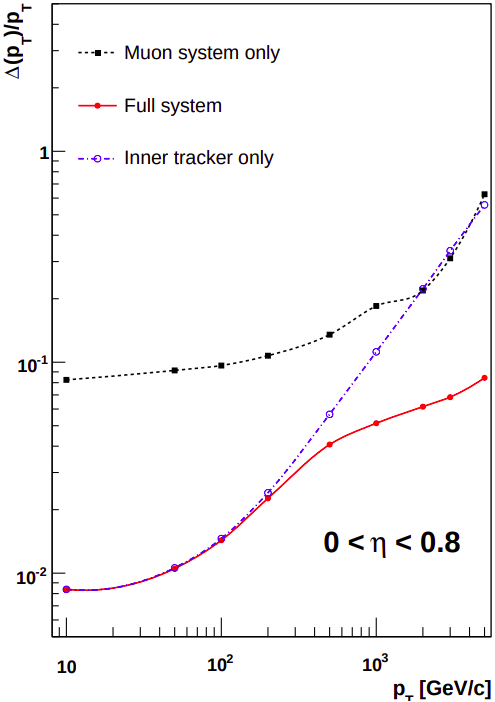
\includegraphics[width=0.5\textwidth]{Figures/muon_res_loweta.png}}
    \subfloat[]{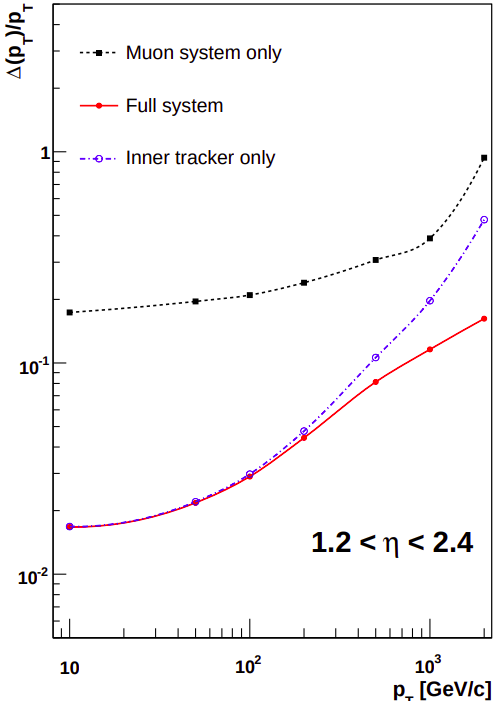
\includegraphics[width=0.5\textwidth]{Figures/muon_res_higheta.png}} \\
\caption{The $\pT$ resolution for muon identification using the muon system (black), the inner tracker (blue), and the full system (red). This is shown for the pseduorapidity regions $0 < \eta < 0.8$ (a) and  $1.2 < \eta < 2.4$ (b).}
\label{fig:muon_eff}
\end{figure}

The \texttt{Medium} muon identification~\cite{CMS:2018rym} is used for the analyses described in subsequent chapters.
The requirements for this identification are:
\begin{enumerate}[i)]
\item The muon is reconstructed by the tracker or global muon reconstruction algorithm.
\item The impact parameters, $d_{xy}$ and $d_{z}$, defined as the distance in the xy and z plane of the closest approach to the \ac{PV}, between the muon track and the primary vertex are restricted as $d_{xy}<0.045$ cm and $d_{z}<0.2$ cm to ensure the muon is associated with the primary vertex.
\item At least 80\% of the tracker hits have to be valid.
\end{enumerate}

In addition, either of the following two sets of criteria must be satisfied:

\begin{enumerate}[i)]
\item The muon is reconstructed by the global muon reconstruction algorithm.
\item The $\chi^2$ divided by the number of degrees of freedom of the global track fit is smaller than 3.
\item The $\chi^2$ of the tracker standalone position match~\cite{CMS:2009fdy} is smaller than 12.
\item The $\chi^2$ of the track kink finder~\cite{CMS:2018rym} is less than 20.
\item The muon segment compatibility is $>$ 0.303.
\end{enumerate}

or,

\begin{enumerate}[i)]
\item The muon segment compatibility is $>$ 0.451 
\end{enumerate}

The efficiency of the \texttt{Medium} muon identification is approximately 90\%, with a misidentification probability of approximately 0.1\%. \\

To reduce the contamination from muons originating from heavy-flavoured quark decays, muons are required to be isolated from hadronic activity in the detector. 
The isolation is based on the $\pT$ of the photon ($\gamma$), neutral ($\text{h}^0$) and charged hadron ($\text{h}^{\pm}$ if originating from the \ac{PV} and $\text{h}^{\pm}, \text{PU}$ if not originating from \ac{PV}) \ac{PF} candidates within a cone size of $\Delta R<0.4$ of the selected muon ($\mu$). 
A relative combined isolation variable is defined as:

\begin{equation}
\label{eqn:reliso}
\Irel = \frac{1}{\pT^{\mu}} \Big( \sum \pT^{\text{h}^{\pm}} + \text{max}\Big( 0, \sum \pT^{\text{h}^0} + \sum \pT^{\gamma} - \Delta \beta \sum \pT^{\text{h}^{\pm}, \text{PU}} \Big) \Big),
\end{equation}

where the sums loop through all objects with the cone and $\Delta \beta$ is the energy estimate of neutral particles due to pileup, which is taken to be 0.5.
This represents an estimated fraction of transverse momenta between the other contributions within the cone that originate from the interaction at the \ac{PV}, and the muon itself.
The muon isolation can then be used to separate muons, with a low value of $\Irel$, from other hadronic objects, at higher values of $\Irel$

\section{Electrons}

In addition to the \ac{PF} algorithm to reconstruct electrons, they are required to pass an identification variable based on a \ac{BDT} discriminator to distinguish genuine electrons from backgrounds like misidentified jets, electrons from photon conversions, and electrons produced in heavy-flavour decays~\cite{CMS:2015xaf}.
The following variables are used as input to the \ac{BDT}:

\begin{enumerate}[i)]
\item Shower shape variables.
\item The fraction of energy deposited in the \ac{HCAL}.
\item The fraction of energy lost through bremsstrahlung.
\item Track quality variables.
\item The variable $1/E_{\text{SC}} - 1/p$, where $E_{SC}$ is the \ac{SC} energy and $p$ is the momentum of the track at the point of closest approach to the vertex.
\item Variables comparing the geometrical matching between the track and the \ac{SC}.
\end{enumerate}

The \ac{BDT} was trained on a $Z/\gamma^{*}$ \ac{MC} sample generated with \MADGRAPH, in 3 $\eta$ bins for electrons with $\pT>10$ GeV.
The performance of the \ac{BDT} is shown in Figure~\ref{fig:electron_eff}.
This thesis uses the version of the identification \ac{BDT} without the isolation included in the training, instead using an additional cut on the electron isolation. 
This allows for easily accessible sideband regions (orthogonal regions to the signal) used for estimation of background estimation. \\

\begin{figure}[t]
\centering
    \subfloat[]{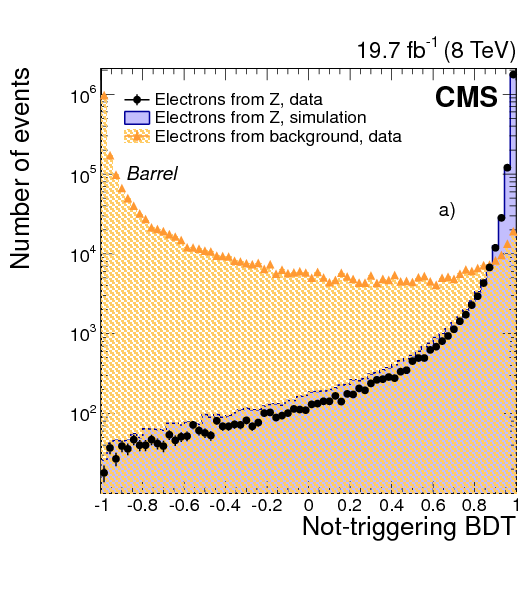
\includegraphics[width=0.5\textwidth]{Figures/electron_id_barrel.png}}
    \subfloat[]{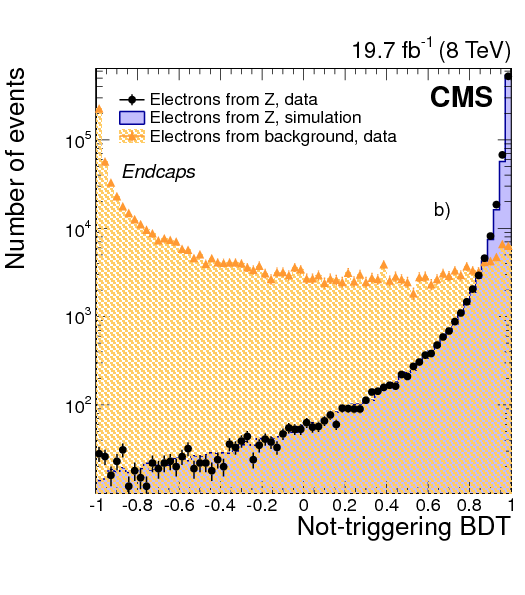
\includegraphics[width=0.5\textwidth]{Figures/electron_id_endcap.png}} \\
\caption{Performance of the electron BDT using $Z\rightarrow ee$ enriched events from data (dots), background-enriched events from data (triangles), and $Z\rightarrow ee$ MC events (purple solid histogram). This is shown for the performance in the barrel (a) and the endcaps (b) for a BDT that does not utilise trigger information during training~\cite{CMS:2015xaf}.}
\label{fig:electron_eff}
\end{figure}

The electron are required to pass the 90\% efficiency working point of the \ac{BDT}, which corresponds to a misidentification probability of 2\%~\cite{CMS:2015xaf}. 
Finally electrons are also subject to the same impact parameter requirements as the muons: the impact parameters $d_{xy}$ and $d_{z}$ between the electron track and the primary vertex are restricted as $d_{xy}<0.045$ cm and $d_{z}<0.2$ cm to ensure the electron is associated with the primary vertex. \\

Similarly to muons, an isolation variable is used to further separate electrons from other backgrounds.
Different to for muons, the isolation used is based on photon, neutral and charged hadron \ac{PF} candidates within a smaller cone size of $\Delta R<0.3$ of the selected electron.
A different method to estimate the neutral particles due to \ac{PU} is used, namely the rho-effective-area method. 
The pileup in this method is estimated as $PU=\rho\cdot A_{\text{eff}}$, where $\rho$ is the event-specific average pile-up energy density per unit area in the $\phi$-$\eta$ plane and the $A_{\text{eff}}$ is the effective area specific to the given type of isolation. 
The rho-effective-area subtracted relative combined isolation variable is defined as

\begin{equation}
\label{eqn:electron_reliso_rho}
\Irel = \frac{1}{\pT^{e}} \Big( \sum \pT^{\text{h}^{\pm}} + \text{max}\Big( 0, \sum \pT^{\text{h}^0} + \sum \pT^{\gamma} - \rho A_{\text{eff}} \Big) \Big),
\end{equation}

where $A_{\text{eff}}$ is measured in bins of $\eta$ as listed in Table~\ref{tab:EleEA}.

\begin{table}[htb]
\begin{center}
\begin{tabular}{|c|c|}
\hline
$\eta$ range & $A_{\text{eff}}$ \\
\hline
\hline
0.0$\leq\eta<$1.0   &  0.1440 \\
1.0$\leq\eta<$1.479 &  0.1562 \\
1.479$\leq\eta<$2.0 &  0.1032 \\
2.0$\leq\eta<$2.2   &  0.0859 \\
2.2$\leq\eta<$2.3   &  0.1116 \\
2.3$\leq\eta<$2.4   &  0.1321 \\
2.4$\leq\eta<$5.0   &  0.1654 \\
\hline
\end{tabular}
\end{center}
\caption{
 Electron effective areas used for the $\rho$-corrected isolation computation~\cite{CMS:2015xaf}.
}
\label{tab:EleEA}
\end{table}

\section{Jets}

Quarks and gluons undergo fragmentation and hadronisation, resulting in collimated sprays of hadrons called jets~\cite{Salam:2010nqg}. 
The process of combining particles into jets is accomplished through the anti-$k_T$ jet clustering algorithm~\cite{Cacciari:2008gp} as implemented in \texttt{FastJet}~\cite{Cacciari:2011ma}. 
This algorithm relies two distance parameters: $d_{ij}$, representing the distance between objects $i$ and $j$, and $d_{iB}$, representing the distance between object $i$ and the beam. 
These objects can be individual particles or clusters of particles. 
The distance parameters are defined as,

\begin{align}
\begin{split}
d_{ij} &= \text{min}(p_{T,i}^{-2}, p_{T,j}^{-2})  \frac{\Delta R_{ij}^{2}}{R^{2}}, \\ 
d_{iB} &= p_{T,i}^{-2}, 
\end{split}
\end{align} 
 
where $\Delta R_{ij}$ is the separation in $\delta R$ of objects i and j, and $R$ is the radius parameter controlling the typical size of the jets. 
The clustering process unfolds as follows:

\begin{enumerate}[i)]
\item Compute the minimum of $d_{ij}$ and $d_{iB}$ for all objects.
\item If the minimum corresponds to $d_{ij}$, merge objects $i$ and $j$ into a single entity.
\item If the minimum corresponds to $d_{iB}$, set object $i$ as a jet and remove it from the object list.
\item Repeat steps (i) to (iii) until no objects remain. 
\end{enumerate}

Chapters~\ref{sec:bsm_H_to_tau_tau_analysis} and \ref{sec:H_A_to_4_tau_analysis} use jets clustered with a radius parameter of $R = 0.4$, often called AK4 jets.
The impact of \ac{PU} on jet energy and substructure is addressed by using the \ac{CHS} technique~\cite{CMS:2017wyc}. 
\ac{CHS} excludes charged hadrons that are not associated with the primary vertex during jet clustering. 
To reject misidentified jets a discriminator evaluated on variables like energy fractions carried by different types of \ac{PF} candidates, as well as charged and neutral particle multiplicities is used~\cite{CMS:2017wyc}. 
For data collected in 2017, the region with $2.65 < |\eta| < 3.139$ experiences substantial \ac{ECAL} noise, leading to a notable increase in the number of jets. 
To veto this, jets with $\pT < 50$ GeV within this $\eta$ range are removed and a \ac{PU} jet identification discriminant~\cite{CMS:2013wea}.
For $\tau$ selections in the later chapters, to exclude selected jets from electon, muon or hadronic tau candidates, the jets are required to be separated from the selected $\tau$ candidate by $\Delta R > 0.5$.

\section{b jets}

For determining whether a jet is initiated by a b quark, the \texttt{DeepJet} algorithm~\cite{CMS:2017wtu,Bols:2020bkb} is used.  
This heavy-flavour jet identifier, uses properties of the jet to distinguish jets originating from b quarks, c quarks, the remainder of the lighter quarks grouped, and gluons.
Core to the b tagging in this algorithm is the reconstruction of a \ac{SV} due to the lifetime of b quarks, allowing for displaced tracks.
The \texttt{DeepJet} \ac{DNN} uses a combination of high-level variables such as the \ac{SV}, as well as utilising low-level variable of jet constituents to separate between initiators.
The \ac{DNN} uses a mixture of convolutional and dense layers to perform this categorisation.
The performance of the algorithm is shown in Figure~\ref{fig:deepjet}.

For b jet selection, jets are required to have $\pT > 20$ GeV and $|\eta| <$ 2.4 (2.5) in 2016 (2017 and 2018), and are considered b tagged if their discriminator value is larger than some threshold that represents a mis-identification rate of 1\%.
This corresponds to a b tagging efficiency around 80\%.

\begin{figure}[!hbtp]
\centering
    \subfloat[]{\includegraphics[width=0.8\textwidth]{Figures/deepjet.pdf}}
\caption{Mis-identification probability 2$\sigma$ bands against efficiency for b tagging using the \texttt{DeepJet} algorithm, for AK4jets with $\pT> 30$ GeV AND $|\eta|$<2.5 utilising MC with parameters from the 2017 era of data taking. Two bands are displayed, one for the identification of a b quark rather than light quarks and gluons (blue) and one for the identification of a b quark rather than a c quark (red)~\cite{deepjet}.}
\label{fig:deepjet}
\end{figure}

\section{Missing transverse energy}

The \ac{MET} is used as a feature to understand particles passing through the \ac{CMS}, such as neutrinos in the \ac{SM}, and weakly interacting particles from hypothetical \ac{BSM} extensions.
This information cannot be pulled from the detector itself but instead the absence of detection can be used to infer the presence of such an object
The \ac{MET} is nominally calculated as the negative vector sum of all transverse momenta of the \ac{PF} candidates in the collision event,

\begin{equation}
\vec{E}_{T}^{\text{miss}} = - \sum_{i} \vec{p}_{T}^{\hspace{4pt}i}.
\end{equation}

However, this raw \ac{PF}\ac{MET} is inaccurate due to the $\pT$ thresholds of the calorimeters, the non-linearity of the calorimeter response and due to reconstruction inefficiencies~\cite{CMS:2016ljj}.
This is fixed with jet energy corrections, determined for jets with $\pT$> 15 GeV and less than 90\% for their energies deposited in the \ac{ECAL} for each of the problems mentioned, and then the corrected \ac{MET} is calculated by,

\begin{equation}
\vec{E}_{T}^{\text{miss,corr}} = \vec{E}_{T}^{\text{miss}} - \sum_{\text{jets}} (\vec{p}_{T,\text{jet}}^{\text{\hspace{4pt}corr}} - \vec{p}_{T,\text{jet}}^{\text{\hspace{4pt}raw}}),
\end{equation}

where \say{corr} and \say{raw} are the corrected and uncorrected values of the jet momenta, respectively. \\

Further corrections are required to account for \ac{PU} effects, and the \texttt{PUPPI} algorithm is used for this purpose~\cite{CMS:2020ebo}.
The algorithm is designed to address the impact of \ac{PU} on observables involving clustered hadrons, such as jets, missing transverse momentum, and lepton isolation. 
It achieves this by combining information about the local particle distribution, event \ac{PU} properties, and tracking data. 
\texttt{PUPPI} operates at the level of individual particle candidates, before any clustering is performed. 
It assigns a weight to each particle, ranging from 0 to 1, based on the information from surrounding particles. 
A weight of 1 is given to particles believed to originate from the \ac{PV}. 
These per-particle weights are then used to rescale the four-momenta of the particles, effectively correcting for the impact of \ac{PU} and so altering the raw calculation of the \ac{MET} to,

\begin{equation}
\vec{E}_{T}^{\text{miss}} = - \sum_{i} w_{i} \cdot \vec{p}_{T}^{\hspace{4pt}i}.
\end{equation}

\section{Taus}
\label{sec:taus}

Fundamental to this thesis is the identification of tau particles.
The tau lepton is measured to have a mean lifetime of \(2.9 \times 10^{-13}\)s. 
This short lifetimes means that the tau lepton is not directly observable in the \ac{CMS} detector.  
In order to detect these particles, it is important to understand how the tau decays. 
Due to the heavy nature of the particle, it does not only decay leptonically, but unlike the muon, it can also decay hadronically.
A list of prominent decays of the tau lepton are shown in the Table~\ref{tab:tau_decay}.
These decays can be split into three groups: the 17.8\% of taus that decay to an electron ($e$), the 17.4\% that decay into a muon ($\mu$), and hadronic tau decays ($\tauh$) that make up the final 64.8\% of tau decays. 
The leptonic decays of the tau can be accounted for by the identification of electrons and muons as discussed in the previous subsection.  \\

\begin{table}[h]
    \centering
    \begin{tabular}{|c|c|}
         \hline
         Decay Mode & Branching Fraction  \\
         \hline
         \hline
         \textbf{Leptonic Decay ($e$, $\mu$)} & \textbf{35.2\%} \\
         $e^- \bar{\nu}_e \nu_\tau $ & 17.8\% \\
         $\mu^- \bar{\nu}_\mu \nu_\tau $ & 17.4\% \\
         \hline
         \textbf{Hadronic Decay ($\tauh$)} & \textbf{64.8\%} \\
         $h^- \pi^0 \nu_\tau $ & 25.9\% \\
         $h^- \nu_\tau$ & 11.5\% \\
         $h^- h^+ h^+ \nu_\tau$ & 9.8\% \\
         $h^- 2\pi^0 \nu_\tau$ & 9.3\% \\
         $h^- h^+ h^- \pi^0 \nu_\tau$ & 4.8\% \\
         other & 3.2\% \\
         \hline
    \end{tabular}
    \caption{Measured branching fractions for the tau lepton. h represents a charged hadron either a pion or a kaon~\cite{ParticleDataGroup:2022pth}.}
    \label{tab:tau_decay}
\end{table}

A two step process is used to identify hadronic taus.
The \ac{HPS} algorithm is used to initially identify hadronic taus based on jets produced by the anti-$k_{\text{T}}$ algorithm with a distance parameter of $\Delta R = 0.4$. 
To capture the energy deposits left by $\pi^0$ candidates in the ECAL, the photon and electron constituents of the jet responsible for seeding the tau reconstruction are assembled into strips. 
All electrons or photons used are required to have $p_{\text{T}} > 0.5$ GeV.
The initial iteration of the \ac{HPS} algorithm used a fixed strip size of $\Delta \eta \times \Delta \phi$ equal to $0.05 \times 0.20$.
However, this technique was updated to a dynamical strip size to account for the multiple scatterings of $e^+ e^-$ products from a $pi^0$ decay, falling outside of the fixed window.
A reliance of the hadronic tau $\pT$ spectrum of the required strip size was observed and so the following iterative algorithm was proposed to resolve this issue.

\begin{enumerate}[i)]
\item The highest $\pT$ electron or photon (not previously grouped into a strip) is used to initiate a new strip.
\item The second highest $\pT$ electron or photon deposition within,
\begin{equation}
  \Delta \eta = f(\pT^{e/\gamma}) + f(\pT^{\text{strip}}), \hspace{1cm} \Delta \phi = g(\pT^{e/\gamma}) + g(\pT^{\text{strip}})
\end{equation}
of the strip is then combined with the strip.
These functions are determined from a fit to hadronic tau MC, so that 95\% of electrons and photons are contained in a single strip.
These fits are shown in Figure~\ref{fig:hps} and correspond to,
\begin{equation}
f(\pT) = 0.20 \pT^{-0.66}, \hspace{1cm} g(\pT) = 0.35 \pT^{-0.71}
\end{equation}
where the $\pT$ is in units of GeV.
These functions have lower and upper caps of 0.05 to 0.3 for $\Delta\phi$ and 0.05 to 0.15 for $\Delta\eta$.
\item Recalculate the strip position using a weight average of the average $\pT$ of all the electron and photon strip constituents.
\begin{equation}
\eta_{\text{strip}} = \frac{1}{\pT^{\text{strip}}} \sum \pT^{e/\gamma} \eta_{e/\gamma}, \hspace{1cm} \phi_{\text{strip}} = \frac{1}{\pT^{\text{strip}}} \sum \pT^{e/\gamma} \phi_{e/\gamma}
\end{equation}
\item Repeat steps ii and iii until no other electron or photon candidate fulfilling condition ii is found.
\end{enumerate}

\begin{figure}[!hbtp]
\centering
    \subfloat[]{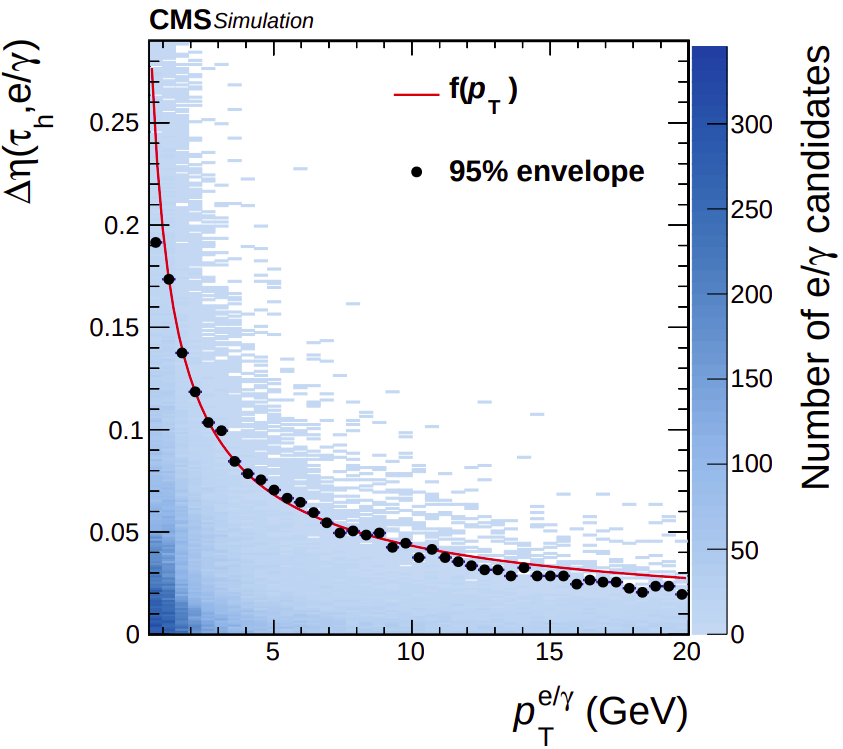
\includegraphics[width=0.5\textwidth]{Figures/hps_f.png}}
    \subfloat[]{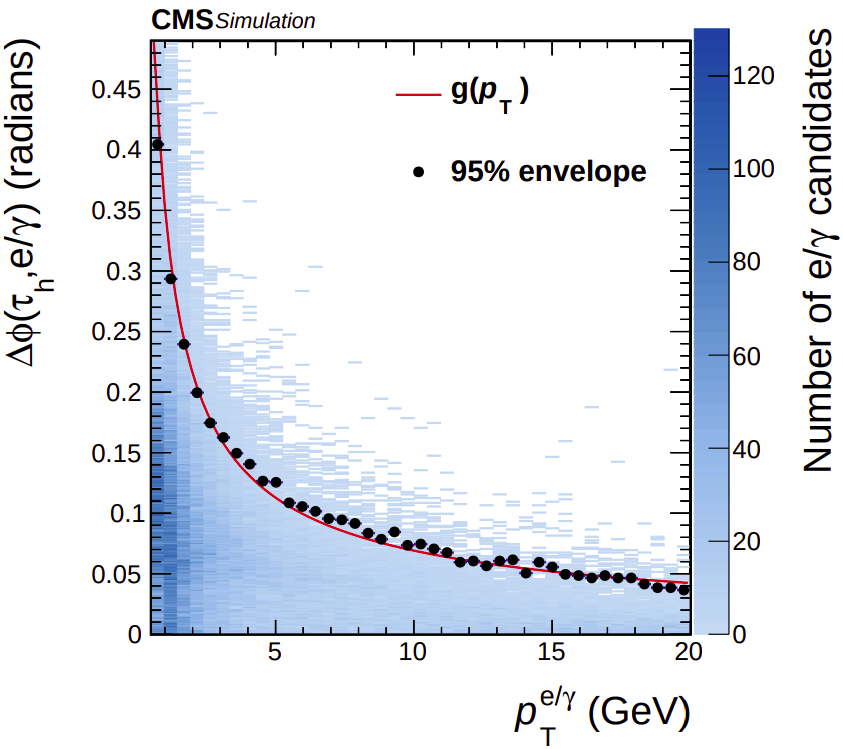
\includegraphics[width=0.5\textwidth]{Figures/hps_g.png}} \\
\caption{The distance between the hadronic tau and electron or photon $\eta$ (a) and $\phi$ (b) with respect the the electron or photon $\pT$. The binned values (points) and the fitted functions $f$ and $g$ (red line), that encapsulates 95\% of all electron and photons are shown in both cases~\cite{Sirunyan:2018pgf}.}
\label{fig:hps}
\end{figure}

Charged hadrons (prongs) are also required to have $\pT > 0.5$ GeV and originate from the \ac{PV}, with a loose transverse impact parameter of $d_{xy} < 0.1$ cm
Further constraints are placed on the reconstructed masses of the specific resonances produced by a hadronic tau decay, if produced by the decay.
In particular, the visible mass positions and widths of the grouped charged hadrons and strips are optimised to match the $\rho$ (770 MeV) and $a_1$ (1260 MeV) decays.
This is performed to maximise the fraction of hadronic tau efficiency to the probability of misidentification from jets.
The visible decay products of each decay shown in Tab~\ref{tab:tau_decay} are reconstructed by:

\begin{enumerate}[i)]
\item $h^- \pi^0$: One charged hadron candidate and no strips.
\item $h^-$: One charged hadron candidate and one strip with mass $ 0.3 < m_{\tau} < 1.3 \sqrt{p_{\text{T}}/100}$ GeV. The mass is required to be between 1.3 and 4.2 GeV.
\item $\pi^- \pi^- \pi^+$: Three charged hadron candidates with mass $0.8 < m_{\tau} < 1.5$ GeV. The tracks are required to originate within $\Delta z<0.4$ cm of the same vertex.
\item $h^- 2\pi^0$: One charged hadron candidate and two strips. The $\tau_{h}$ mass should be $0.4 < m_{\tau} < 1.2\sqrt{p_{\text{T}}/100}$~GeV. The mass is required to be between 1.2 and 4.0 GeV.
\item $\pi^- \pi^- \pi^+ \pi^0$: Three charged hadron candidates and one strip.
\end{enumerate}

The remaining hadronic decays of the tau leptons are not included in this thesis.
The \ac{DM} of the hadronic tau that is reconstructed by a \ac{HPS} is quantified by the following formula relating the number of charged hadron candidates $N_C$ and the number of strips $N_N$.

\begin{equation}
\text{DM} = 5(N_{C} - 1) + N_{N}
\end{equation}

The second step of the identification, comes from a multiclass \ac{DNN}-based algorithm named \texttt{DeepTau}, that seeks to discriminate hadronic tau decays from electron, muons, and most importantly quark or gluon jets, that can be misidentified as hadronic tau decays~\cite{CMS:2022prd}.
It uses a \ac{DNN} architecture that consists of multiple interconnected layers of nodes, that attempts to learn whether the input object is an hadronic tau decay, an electron, a muon or a jet. 
The algorithm takes inputs from reconstructed particles surrounding the \ac{HPS} hadronic tau candidate, including information about energies, momenta, and spatial positions. 
Convolutional layers are used to efficiently process these inputs by dividing them into smaller regions in $\eta$-$\phi$ space, which allows the algorithm to extract local patterns and features. 
It also incorporates high-level features of the hadronic tau candidate calculated from the \ac{HPS} algorithm, such as the four-momentum, charge, \ac{DM}, isolation variables used in previous \ac{MVA}~\cite{CMS:2018jrd}, impact parameters, $\eta$ and $\phi$ strip information, as well as event level information such as variables related to the $\ac{PU}$.
The architecture of algorithm is shown in Figure~\ref{fig:deeptau}. \\

\begin{figure}[!hbtp]
\centering
    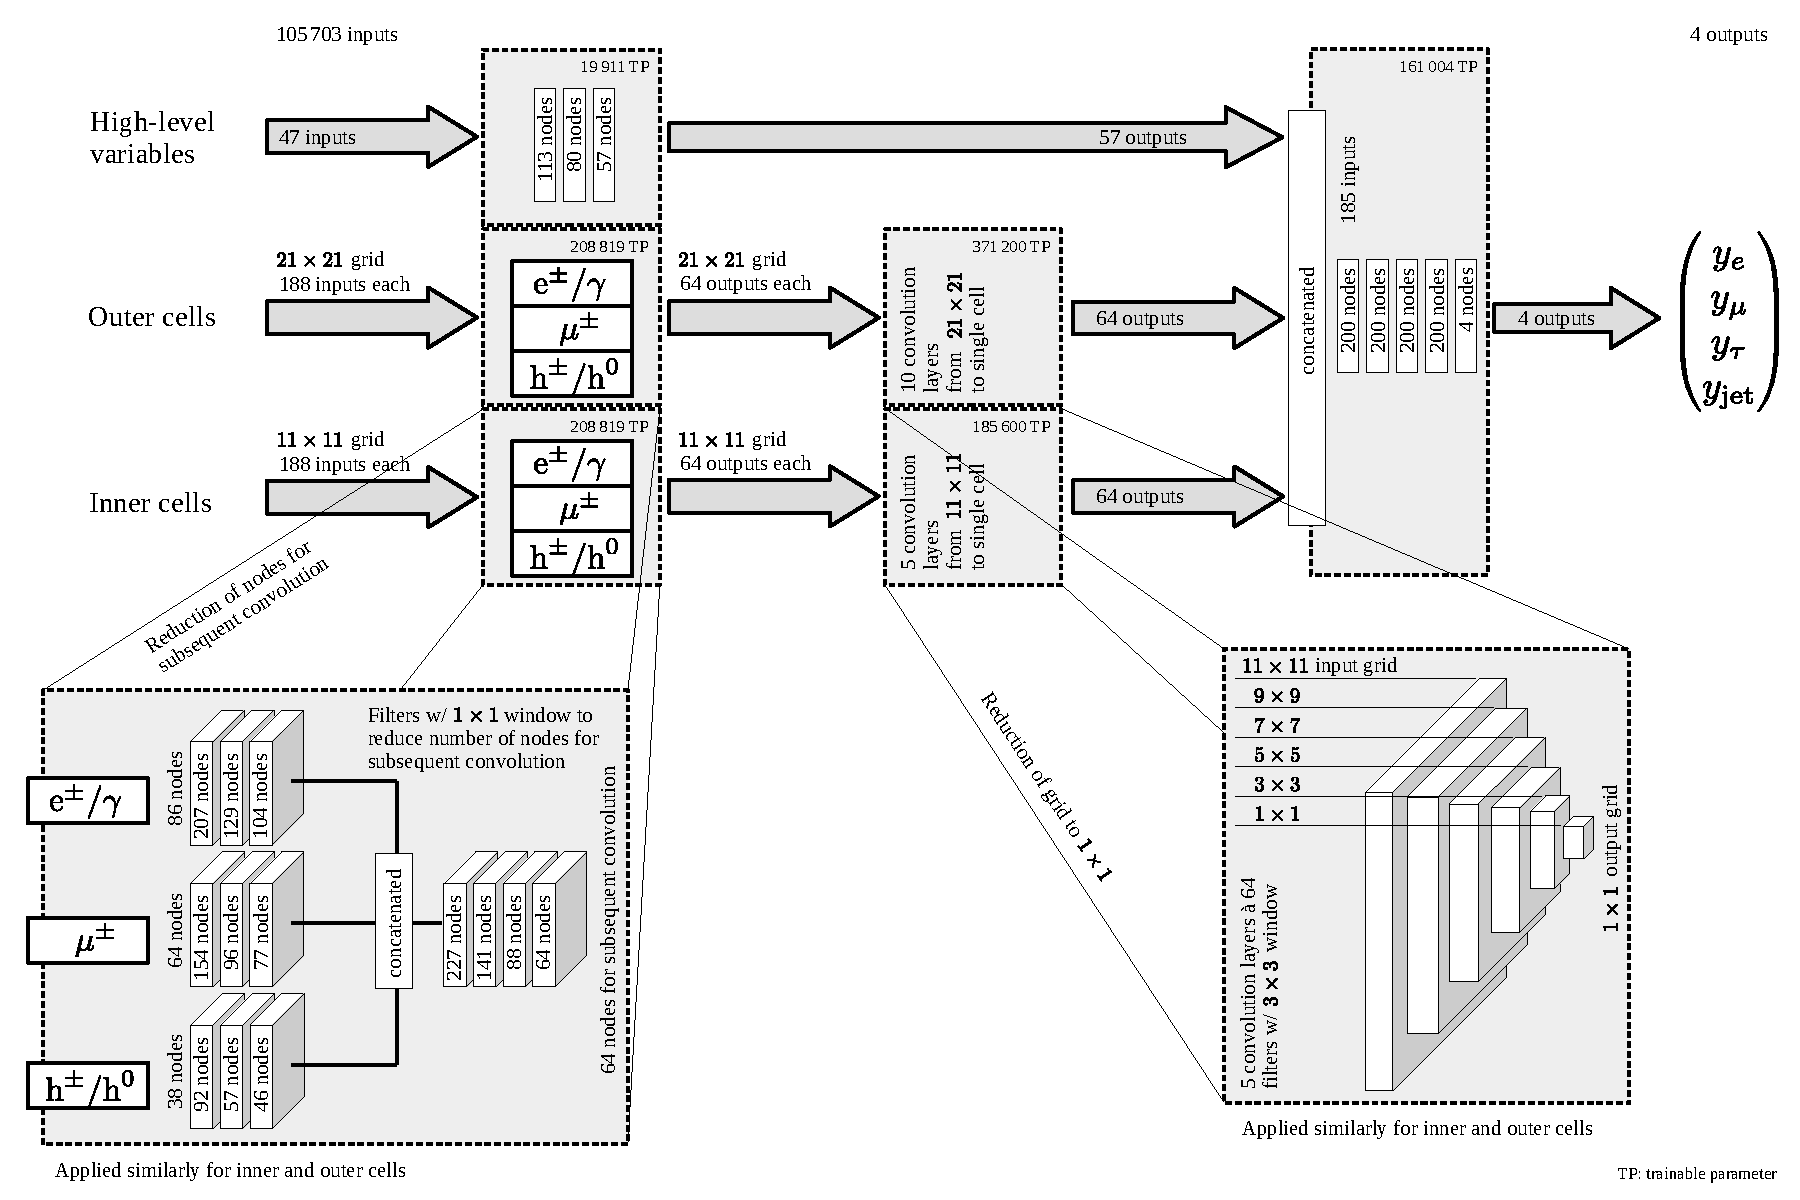
\includegraphics[width=\textwidth]{Figures/deeptau.pdf}
\caption{The architecture of the \texttt{DeepTau} neural network, comprising of three sets of input variables: inner cells, outer cells, and high-level features. These sets are processed separately through subnetworks and their outputs are concatenated. Five fully connected layers process the concatenated output to calculate the probabilities for a candidate to be a hadronic tau, electron, muon, or jet. The high-level input subnetwork consists of three fully connected layers, taking 47 inputs and yielding 57 outputs. Complex subnetworks process the features of inner and outer cells separately, with fully connected layers followed by concatenation and additional fully connected layers. Convolutional layers progressively reduce the grid size for both inner and outer cells. For inner cells, there are 5 convolutional layers, while for outer cells, there are 10 convolutional layers. The number of trainable parameters (TP) for the different subnetworks are also provided~\cite{CMS:2022prd}.}
\label{fig:deeptau}
\end{figure}

The \texttt{DeepTau} \ac{DNN} is trained using a large dataset, incorporating examples of hadronic tau decays and background processes of electrons, muons and jets. 
The output of the \ac{DNN} is 4 scores, that represent the probability that the object is a hadronic tau ($y_\tau$), an electon ($y_e$), a muon ($y_\mu$) or a jet ($y_{\text{jet}}$).
From these raw scores, additional scores are calculated for the probability that an object is a hadronic tau rather than an electron, muon or jet.
These are defined as,

\begin{equation}
D_{i}^{\text{score}} = \frac{y_\tau}{y_i + y_{\tau}}, \hspace{1cm} i \in (e,\mu,\text{jet}).
\end{equation}

From this, \ac{WP}s are defined to match specific efficiencies of hadronic tau identification with respect to each of the other 3 objects, named $D_{e}^{\text{WP}}$, $D_{\mu}^{\text{WP}}$ and $D_{\text{jet}}^{\text{WP}}$.
The target efficiencies for different \ac{WP} are shown in Table~\ref{tab:deeptau_eff}. \\

\begin{table}[!hbtp]
\begin{adjustwidth}{-1cm}{-1cm}
\centering
\begin{tabular}{|c|cccccccc|}
\hline
WP                     & VVTight & VTight & Tight  & Medium & Loose  & VLoose  & VVLoose & VVVLoose \\
\hline 
\hline
$D_{e}^{\text{WP}}$    & 60\%    & 70\%   & 80\%   & 90\%   & 95\%   & 98\%    & 99\%    & 99.5\%   \\
$D_{\mu}^{\text{WP}}$  & -       & -      & 99.5\% & 99.8\% & 99.9\% & 99.95\% & -       & -        \\
$D_{\tau}^{\text{WP}}$ & 40\%    & 50\%   & 60\%   & 70\%   & 80\%   & 90\%    & 95\%    & 98\%     \\
\hline
\end{tabular}
\caption{Target efficiencies of the \texttt{DeepTau} working points with respect to electrons, muons and jets.}
\label{tab:deeptau_eff}
\end{adjustwidth}
\end{table}

Due to the lack of muons misidentified as hadronic taus, high efficiencies can be required for $D_{\mu}^{\text{WP}}$.
This is also the reason for why the target efficiencies for $D_{e}^{\text{WP}}$ are higher than for $D_{\text{jet}}^{\text{WP}}$, where the large challenge jets misidentified as hadronic taus is present.
The misidentification probabilities for the different hadronic tau efficiencies are shown in Figure~\ref{fig:deeptau_misid}.
Also shown in these plots, is the performance comparison to an older \ac{MVA} algorithm for electrons and jets, as well as a cut based algorithm for muons, both described in Reference~\cite{CMS:2018jrd}.
Significant improvements with respect to the previous algorithm is observed, which has a results in a significant improvement in analyses utilising tau leptons at the CMS experiment.
The different $D_{e}^{\text{WP}}$, $D_{\mu}^{\text{WP}}$ and $D_{\text{jet}}^{\text{WP}}$ can be used to optimise the hadronic tau identification for analyses attempting to separate tau enriched signals from backgrounds of misidentified objects.
Two examples of analyses that utilise this are described in Chapter~\ref{sec:bsm_H_to_tau_tau_analysis} and \ref{sec:H_A_to_4_tau_analysis}.

\begin{figure}[!hbtp]
\centering
    \subfloat[]{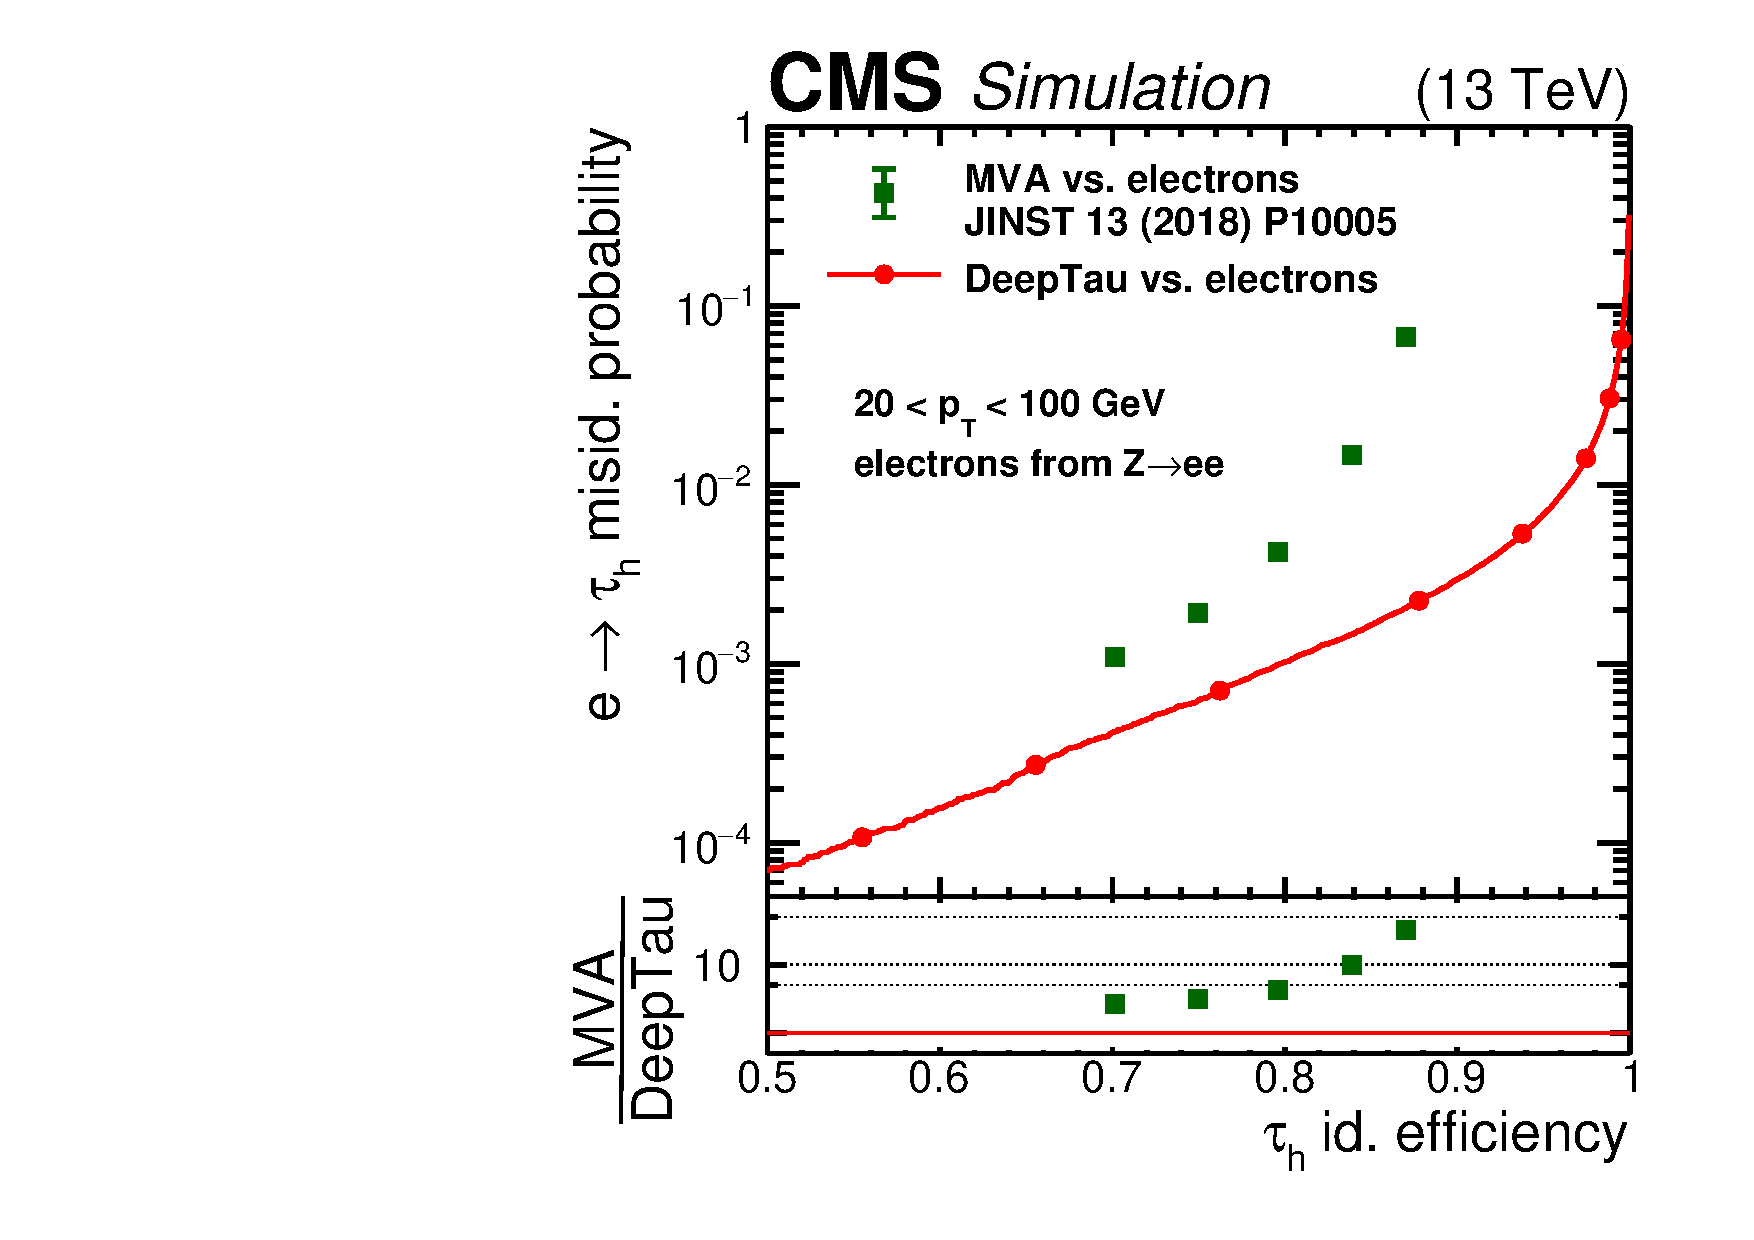
\includegraphics[width=0.5\textwidth]{Figures/deeptau_misid_electron.pdf}}
    \subfloat[]{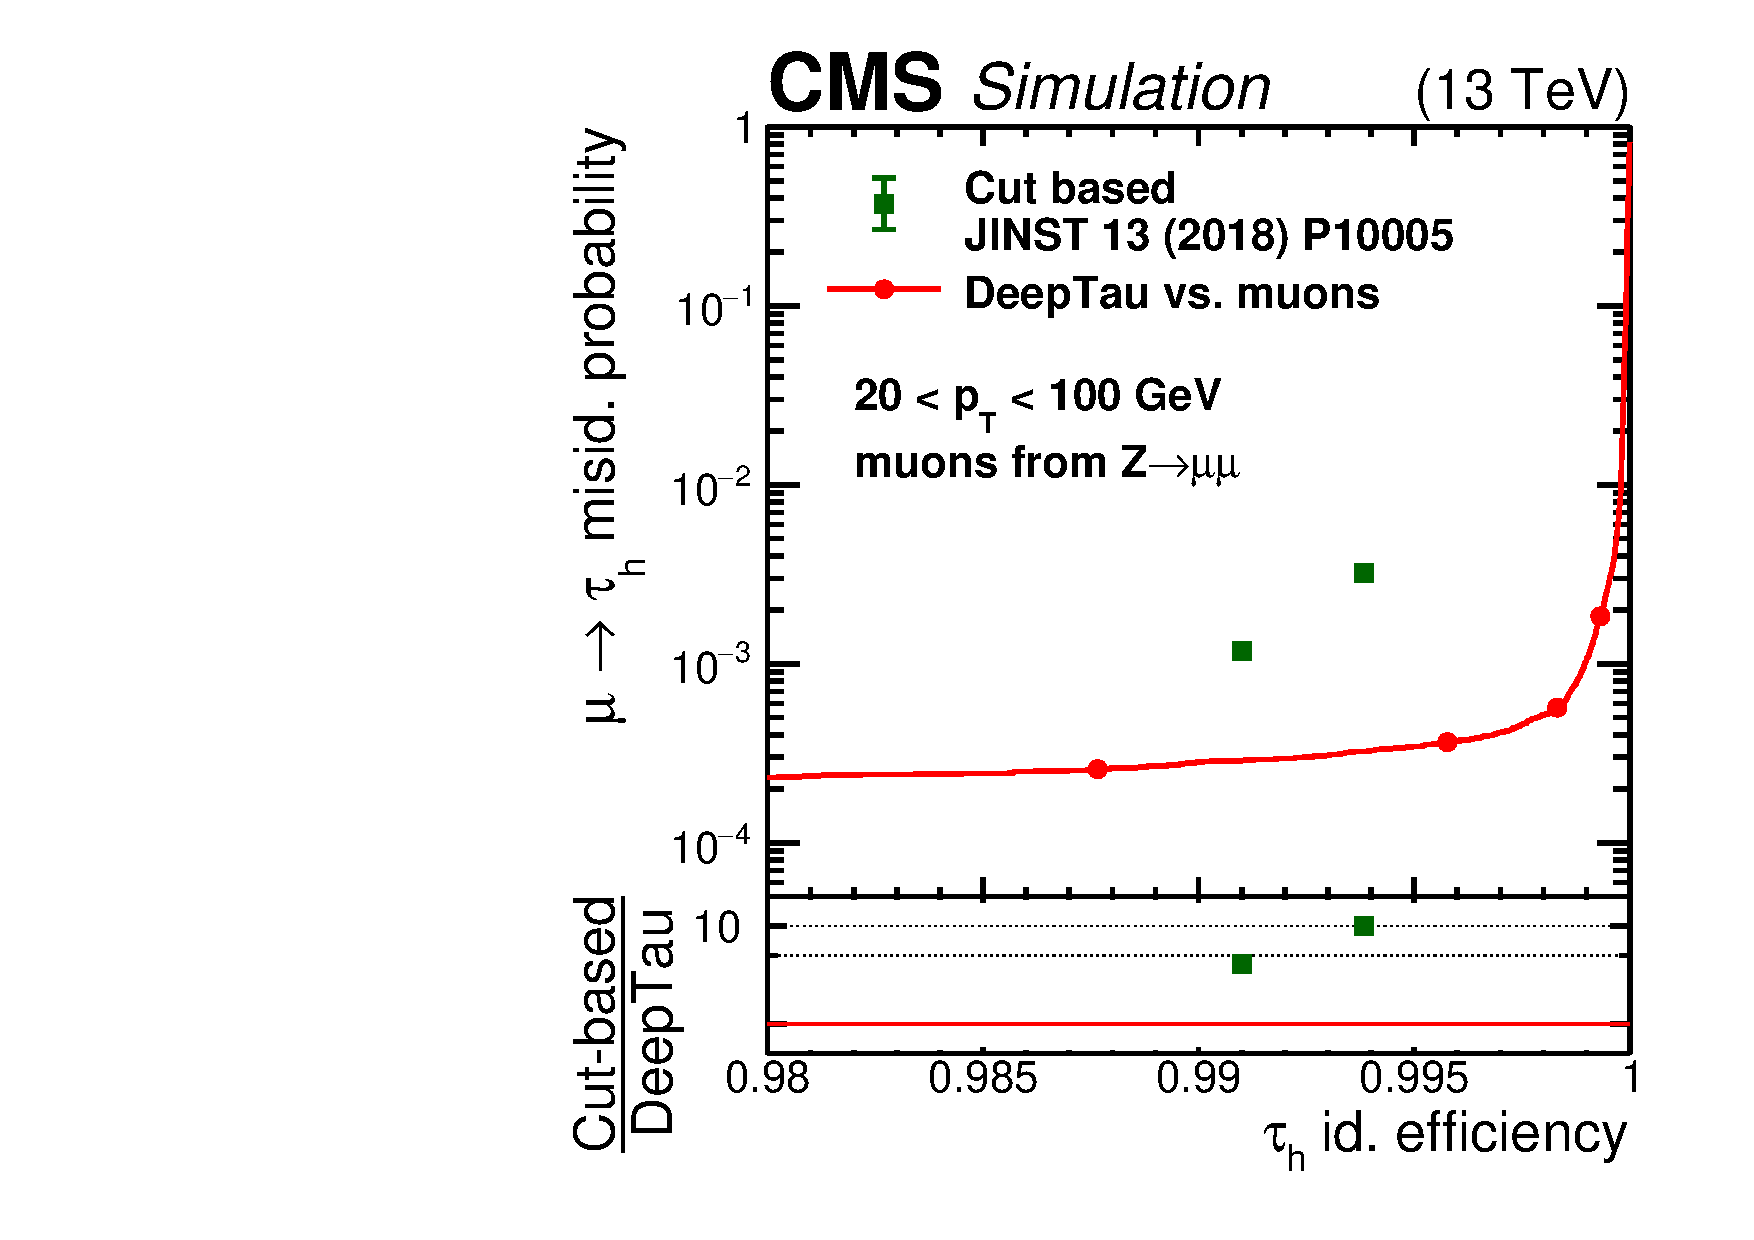
\includegraphics[width=0.5\textwidth]{Figures/deeptau_misid_muon.pdf}} \\
    \subfloat[]{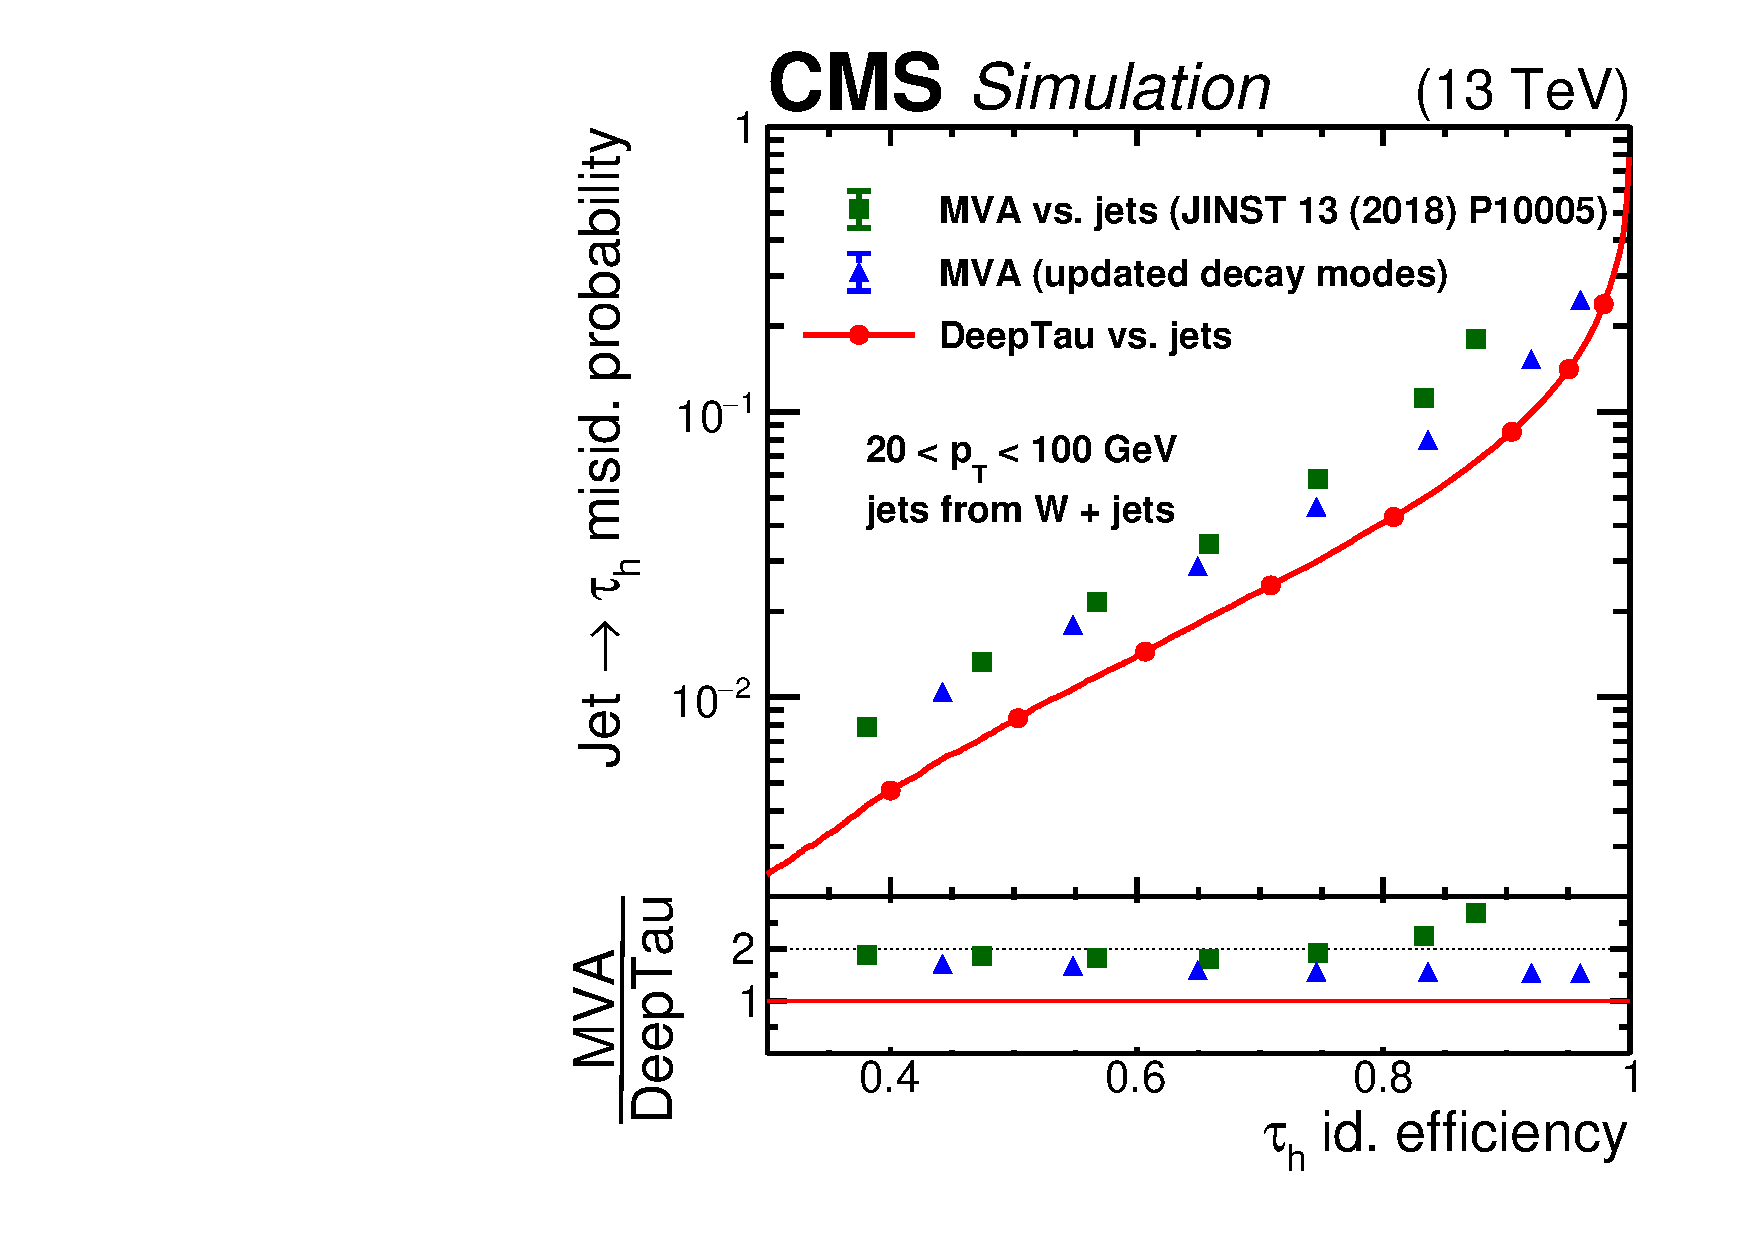
\includegraphics[width=0.5\textwidth]{Figures/deeptau_misid_jet.pdf}}
\caption{Efficiency comparisons of electrons (a), muons (b) and jets (c) passing the \texttt{DeepTau} identification discriminators versus hadronic tau efficiency. (a) uses $Z\rightarrow ee$, (b) uses $Z\rightarrow \mu\mu$ and (c) uses W+jets MC, with only objects with $\pT<100$ GeV used. Working points are indicated by full circles and previous algorithms described in Reference~\cite{CMS:2018jrd} are shown in blue triangles and green squares~\cite{CMS:2022prd}.}
\label{fig:deeptau_misid}
\end{figure}
